% Supplementary Information Section
\section*{Supplementary Information}

% Use S-numbering for figures, tables, and equations
\renewcommand{\thefigure}{S\arabic{figure}}
\renewcommand{\thetable}{S\arabic{table}}
\renewcommand{\theequation}{S\arabic{equation}}

% Reset counters
\setcounter{figure}{0}
\setcounter{table}{0}
\setcounter{equation}{0}



\subsection*{Table S1: Organic Precursor Deposition Parameters}
\begin{table}[htbp]
  \centering
  \caption{Optimized molecular layer deposition parameters for each organic precursor.}
  \label{tab:S1_precursors}
  \resizebox{\textwidth}{!}{
  \begin{tabular}{lcccccc}
    \toprule
    \textbf{Organic Precursor} & \textbf{Chamber Temp. (°C)} & \textbf{Organic Temp. (°C)} & \textbf{N$_2$ Overlap (s)} & \textbf{Pump Overlap (s)} & \textbf{Dose (s)} & \textbf{Purge (s)} \\
    \midrule
    Ethane-1,2-diol (EG)               & 120 & [EG Temp.]  & [N$_2$ overlap] & [Pump overlap] & [Dose] & 300 \\
    \textit{cis}-2-Butene-1,4-diol (CB)& 120 & [CB Temp.]  & [N$_2$ overlap] & [Pump overlap] & [Dose] & 300 \\
    2-Methylene-1,3-propanediol (MPD)  & 120 & [MPD Temp.] & [N$_2$ overlap] & [Pump overlap] & [Dose] & 300 \\
    1,3,4-Trihydroxybenzene (THB)      & 120 & 65          & [N$_2$ overlap] & [Pump overlap] & [Dose] & 300 \\
    1,4-Butynediol (BTY)               & 120 & 60          & [N$_2$ overlap] & [Pump overlap] & [Dose] & 300 \\
    3,4-Dihydroxy-1-butene (DHB)       & 120 & [DHB Temp.] & [N$_2$ overlap] & [Pump overlap] & [Dose] & 300 \\
    \bottomrule
  \end{tabular}}
\end{table}

\vspace{1ex}
\noindent\textit{Note:} Precise values of N$_2$ overlap, pump overlap, and organic precursor doses were optimized individually based on precursor volatility and deposition performance.

\subsection*{Table S2: Typical MLD Cycle Sequence Parameters}
\begin{table}[htbp]
  \centering
  \caption{General sequence parameters used in molecular layer deposition cycles.}
  \label{tab:S2_mld_params}
  \begin{tabular}{lccc}
    \toprule
    \textbf{Step} & \textbf{Temperature (°C)} & \textbf{Pressure (mTorr)} & \textbf{Duration (s)} \\
    \midrule
    N$_2$ purge          & 120 & 200 & 300 \\
    TMA/DEZ dose         & 120 & 200 & [\emph{t\textsubscript{inorg}}] \\
    N$_2$ overlap        & 120 & 200 & [\emph{t\textsubscript{overlap}}] \\
    Pump down            & 120 & 50  & [\emph{t\textsubscript{pump}}] \\
    Organic dose         & 120 & 200 & [\emph{t\textsubscript{org}}] \\
    Shared purge         & 120 & 200 & 300 \\
    \bottomrule
  \end{tabular}
\end{table}

\vspace{1ex}
\noindent\textit{Notes:} Durations for organic and inorganic precursor dosing steps were adjusted based on precursor-specific requirements.

\subsection*{Table S3: XPS O~1s Peak Fitting Results}
\begin{table}[htbp]
\centering
\caption{Peak positions and relative areas for O~1s XPS spectra across bonding environments.}
\resizebox{\textwidth}{!}{%
  \begin{tabular}{lcc|cc|cc}
    \toprule
    & \multicolumn{2}{c}{Al–O–Al (Lattice O)} 
    & \multicolumn{2}{c}{Al–O–C (Hydroxyl O)} 
    & \multicolumn{2}{c}{Adsorbed/Oxidized O} \\
    \cmidrule(lr){2-3} \cmidrule(lr){4-5} \cmidrule(lr){6-7}
    Sample 
      & Peak Position (eV) & \% Area
      & Peak Position (eV) & \% Area
      & Peak Position (eV) & \% Area \\
    \midrule
    As Deposited     
      & 530.9 & 27.7 
      & 532.0 & 68.8 
      & 533.5 & 3.5 \\
    Water Exposed    
      & 530.7 & 36.1
      & 532.0 & 57.3
      & 533.1 & 6.6 \\
    Water Exposed UV 
      & 531.0 & 24.8
      & 532.1 & 72.4
      & 533.9 & 2.9 \\
    \bottomrule
  \end{tabular}}
\end{table}

\subsection*{Table S4: XPS C~1s Peak Fitting Results}
\begin{table}[htbp]
\centering
\caption{Peak positions and relative areas for C~1s XPS spectra across bonding environments.}
\resizebox{\textwidth}{!}{%
  \begin{tabular}{lcc|cc|cc|cc|cc}
    \toprule
    & \multicolumn{2}{c}{C–C/C–H (fit1)} 
    & \multicolumn{2}{c}{C–O (fit2)} 
    & \multicolumn{2}{c}{C=O (fit3)} 
    & \multicolumn{2}{c}{Carbonate/Oxidized (fit4)} 
    & \multicolumn{2}{c}{Highly Oxidized (fit5)} \\
    \cmidrule(lr){2-11}
    Sample 
      & Peak (eV) & \% Area
      & Peak (eV) & \% Area
      & Peak (eV) & \% Area
      & Peak (eV) & \% Area
      & Peak (eV) & \% Area \\
    \midrule
    As Deposited     
      & 284.8 & 61.6 & 286.7 & 35.0 & 288.6 & 3.4 & – & – & – & – \\
    Water Exposed    
      & 284.8 & 55.9 & 286.1 & 18.3 & 287.4 & 9.2 & 289.3 & 7.0 & 290.6 & 9.7 \\
    Water Exposed UV 
      & 284.9 & 68.8 & 286.4 & 17.2 & 287.6 & 6.4 & 289.1 & 5.2 & 290.5 & 2.3 \\
    \bottomrule
  \end{tabular}}
\end{table}

\subsection*{Table S5: XPS Al~2p Peak Fitting Results}
\begin{table}[htbp]
\centering
\caption{Peak positions and relative areas for Al~2p XPS spectra across bonding environments.}
\resizebox{0.6\textwidth}{!}{%
  \begin{tabular}{lcc|cc}
    \toprule
    & \multicolumn{2}{c}{Primary Al (fit1)} 
    & \multicolumn{2}{c}{Oxidized/Hydrolyzed Al (fit2)} \\
    \cmidrule(lr){2-5}
    Sample 
      & Peak Position (eV) & \% Area
      & Peak Position (eV) & \% Area \\
    \midrule
    As Deposited     
      & 74.6 & 100.0 & – & – \\
    Water Exposed    
      & 74.6 & 81.9 & 75.5 & 18.1 \\
    Water Exposed UV 
      & 74.6 & 100.0 & – & – \\
    \bottomrule
  \end{tabular}}
\end{table}

\subsection*{Figure S1: EBL Pattern Layouts}
\begin{figure}[htbp]
  \centering
  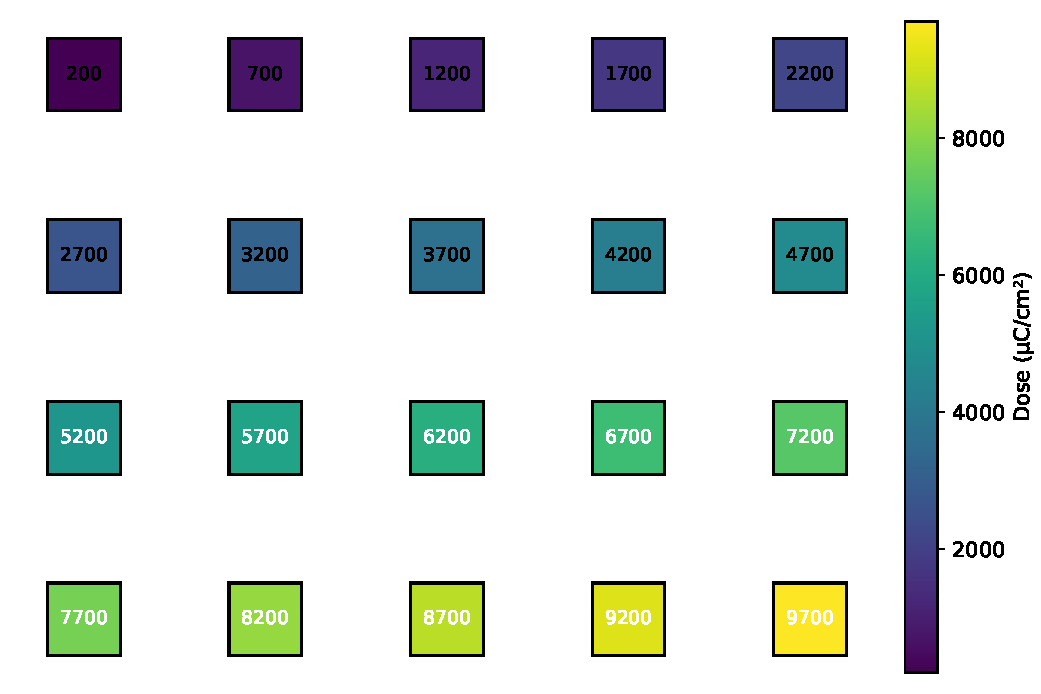
\includegraphics[width=0.7\linewidth]{Figures/dose_matrix_mockup_clean.pdf}
  \caption{Mockup of the electron beam lithography dose matrix. Each square represents a dose from 200 to 9700~\si{\micro\coulomb\per\centi\meter\squared}, color-coded for visualization.}
  \label{fig:dosematrix}
\end{figure}

\subsection*{Figure S2: Grating and Test Region Layout}
\begin{figure}[htbp]
  \centering
  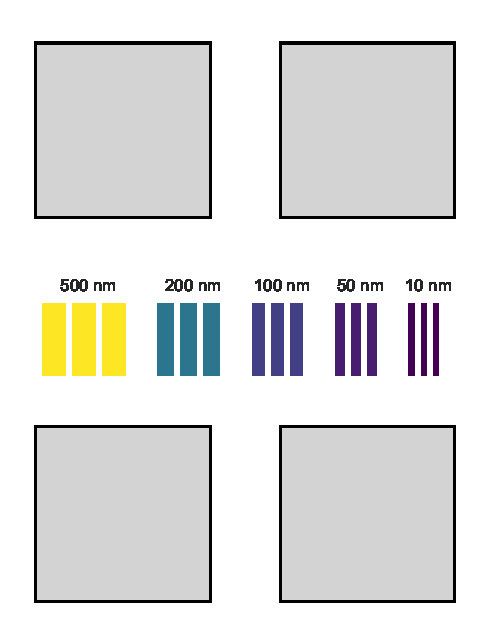
\includegraphics[width=0.7\linewidth]{Figures/box_grating_mockup_clean.pdf}
  \caption{Mockup of four resist test regions surrounding a centered line-space grating array. Each grating group contains three lines of fixed visual width representing target linewidths from 500~nm to 10~nm. Grating bars are color-coded using the Viridis colormap to aid visual differentiation. This layout replicates the spatial structure of GDS files used for resolution and exposure testing.}
  \label{fig:sfig:grating}
\end{figure}


\subsection*{Randomization and Control Scripts}
Substrate randomization and reactor scheduling scripts are available at:  
\url{https://github.com/BergsmanGroup/MLD_high_throughput}
